\documentclass[a4paper,12pt]{article}
\usepackage[margin=18mm]{geometry}
\usepackage{tikz}
\usepackage{amsmath}
\newcommand{\pFourCell}[1]{\makebox[2.7em][c]{\ensuremath{#1}}}
\pagestyle{empty}
\begin{document}
\section*{Spaltentreue LaTeX-Ausgabe}
\noindent Gleichung: \texttt{2*sqrt(x+3)=5} \hfill Zielvariable: \texttt{x}

\vspace{8mm}
\begin{center}
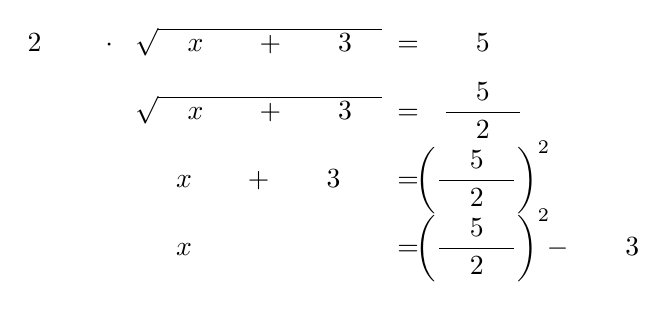
\begin{tikzpicture}[x=2.7em,y=-1em]
\node[anchor=base, inner sep=0pt] at (1,1) {$2$};
\node[anchor=base, inner sep=0pt] at (2,1) {$\cdot$};
\node[anchor=base, inner sep=0pt] at (4,1) {$\sqrt{\pFourCell{x}\pFourCell{+}\pFourCell{3}}$};
\node[anchor=base, inner sep=0pt] at (6,1) {$=$};
\node[anchor=base, inner sep=0pt] at (7,1) {$5$};
\node[anchor=base, inner sep=0pt] at (7,3.45) {$\displaystyle\frac{\pFourCell{5}}{\pFourCell{2}}$};
\node[anchor=base, inner sep=0pt] at (4,3.45) {$\sqrt{\pFourCell{x}\pFourCell{+}\pFourCell{3}}$};
\node[anchor=base, inner sep=0pt] at (6,3.45) {$=$};
\node[anchor=base, inner sep=0pt] at (3,5.9) {$x$};
\node[anchor=base, inner sep=0pt] at (4,5.9) {$+$};
\node[anchor=base, inner sep=0pt] at (5,5.9) {$3$};
\node[anchor=base, inner sep=0pt] at (6,5.9) {$=$};
\node[anchor=base, inner sep=0pt] at (7,5.9) {$\left(\displaystyle\frac{\pFourCell{5}}{\pFourCell{2}}\right)^{2}$};
\node[anchor=base, inner sep=0pt] at (3,8.350000000000001) {$x$};
\node[anchor=base, inner sep=0pt] at (6,8.350000000000001) {$=$};
\node[anchor=base, inner sep=0pt] at (7,8.350000000000001) {$\left(\displaystyle\frac{\pFourCell{5}}{\pFourCell{2}}\right)^{2}$};
\node[anchor=base, inner sep=0pt] at (8,8.350000000000001) {$-$};
\node[anchor=base, inner sep=0pt] at (9,8.350000000000001) {$3$};
\end{tikzpicture}
\end{center}

\newpage
\section*{Spaltentreue LaTeX-Ausgabe mit Raster}
\vspace{6mm}
\begin{center}
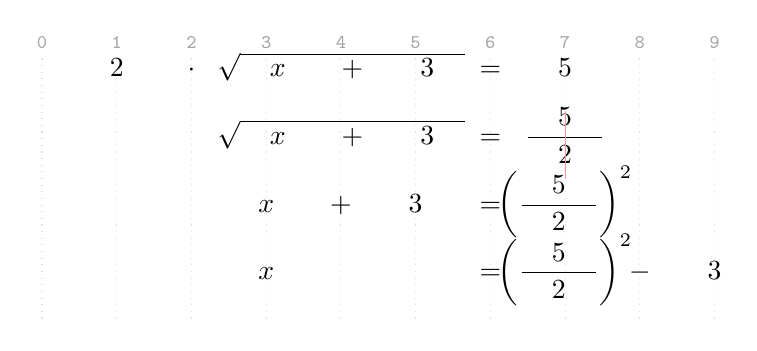
\begin{tikzpicture}[x=2.7em,y=-1em]
\draw[gray!25, dotted] (0,0.35) -- (0,9.900000000000002);
\node[font={\ttfamily\scriptsize}, text=gray!70, anchor=base] at (0,0) {0};
\draw[gray!25, dotted] (1,0.35) -- (1,9.900000000000002);
\node[font={\ttfamily\scriptsize}, text=gray!70, anchor=base] at (1,0) {1};
\draw[gray!25, dotted] (2,0.35) -- (2,9.900000000000002);
\node[font={\ttfamily\scriptsize}, text=gray!70, anchor=base] at (2,0) {2};
\draw[gray!25, dotted] (3,0.35) -- (3,9.900000000000002);
\node[font={\ttfamily\scriptsize}, text=gray!70, anchor=base] at (3,0) {3};
\draw[gray!25, dotted] (4,0.35) -- (4,9.900000000000002);
\node[font={\ttfamily\scriptsize}, text=gray!70, anchor=base] at (4,0) {4};
\draw[gray!25, dotted] (5,0.35) -- (5,9.900000000000002);
\node[font={\ttfamily\scriptsize}, text=gray!70, anchor=base] at (5,0) {5};
\draw[gray!25, dotted] (6,0.35) -- (6,9.900000000000002);
\node[font={\ttfamily\scriptsize}, text=gray!70, anchor=base] at (6,0) {6};
\draw[gray!25, dotted] (7,0.35) -- (7,9.900000000000002);
\node[font={\ttfamily\scriptsize}, text=gray!70, anchor=base] at (7,0) {7};
\draw[gray!25, dotted] (8,0.35) -- (8,9.900000000000002);
\node[font={\ttfamily\scriptsize}, text=gray!70, anchor=base] at (8,0) {8};
\draw[gray!25, dotted] (9,0.35) -- (9,9.900000000000002);
\node[font={\ttfamily\scriptsize}, text=gray!70, anchor=base] at (9,0) {9};
\node[anchor=base, inner sep=0pt] at (1,1) {$2$};
\node[anchor=base, inner sep=0pt] at (2,1) {$\cdot$};
\node[anchor=base, inner sep=0pt] at (4,1) {$\sqrt{\pFourCell{x}\pFourCell{+}\pFourCell{3}}$};
\node[anchor=base, inner sep=0pt] at (6,1) {$=$};
\node[anchor=base, inner sep=0pt] at (7,1) {$5$};
\node[anchor=base, inner sep=0pt] at (7,3.45) {$\displaystyle\frac{\pFourCell{5}}{\pFourCell{2}}$};
\draw[red!40, line width=0.35pt] (7,2.25) -- (7,4.7);
\node[anchor=base, inner sep=0pt] at (4,3.45) {$\sqrt{\pFourCell{x}\pFourCell{+}\pFourCell{3}}$};
\node[anchor=base, inner sep=0pt] at (6,3.45) {$=$};
\node[anchor=base, inner sep=0pt] at (3,5.9) {$x$};
\node[anchor=base, inner sep=0pt] at (4,5.9) {$+$};
\node[anchor=base, inner sep=0pt] at (5,5.9) {$3$};
\node[anchor=base, inner sep=0pt] at (6,5.9) {$=$};
\node[anchor=base, inner sep=0pt] at (7,5.9) {$\left(\displaystyle\frac{\pFourCell{5}}{\pFourCell{2}}\right)^{2}$};
\node[anchor=base, inner sep=0pt] at (3,8.350000000000001) {$x$};
\node[anchor=base, inner sep=0pt] at (6,8.350000000000001) {$=$};
\node[anchor=base, inner sep=0pt] at (7,8.350000000000001) {$\left(\displaystyle\frac{\pFourCell{5}}{\pFourCell{2}}\right)^{2}$};
\node[anchor=base, inner sep=0pt] at (8,8.350000000000001) {$-$};
\node[anchor=base, inner sep=0pt] at (9,8.350000000000001) {$3$};
\end{tikzpicture}
\end{center}
\end{document}
